\documentclass{beamer}
%% Possible paper sizes: a0, a0b, a1, a2, a3, a4.
%% Possible orientations: portrait, landscape
%% Font sizes can be changed using the scale option.
% \usepackage[size=a3,orientation=landscape,scale=1.8]{beamerposter}
\usepackage[size=custom,width=80,height=128,scale=1.1]{beamerposter}
\usetheme{LLT-poster}
% \usecolortheme{ComingClean}
\usecolortheme{Entrepreneur}
% \usecolortheme{ConspicuousCreep}  %% VERY garish.

\usepackage[utf8]{inputenc}
\usepackage[T1]{fontenc}
\usepackage{libertine}
\usepackage[scaled=0.92]{inconsolata}
\usepackage[libertine]{newtxmath}
\usepackage{natbib}
\bibliographystyle{plain}
\renewcommand*{\bibfont}{\tiny}
\newcommand{\paragraph}[1]{\noindent\textbf{#1}\quad}

\usepackage{mwe}

\author[ivan.puhachov@umontreal.ca]{Ivan Puhachov}
\title{Generative Vector Art}
\institute{Universite de Montreal}
% Optional foot image
%\footimage{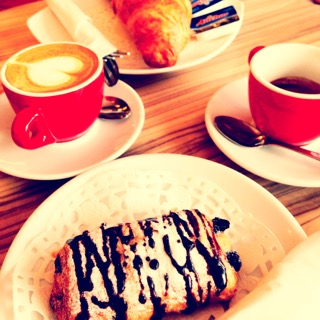
\includegraphics[width=4cm]{IMG_1934.jpg}}

\begin{document}
\begin{frame}[fragile]
	\begin{center}
		\vspace{5mm}
		
		{\LARGE Universite de Montreal}
		\vspace{7mm}
		
		{\LARGE IFT6756}\vspace{7mm}
		
		{\LARGE Ivan Puhachov}
	\end{center}
\begin{block}{}
	\begin{center}
	
\includegraphics[width=0.45\linewidth]{images/my_plot_vector.png}
	\hspace{1cm}
	\unskip\ \vrule\
	\hspace{1cm}
	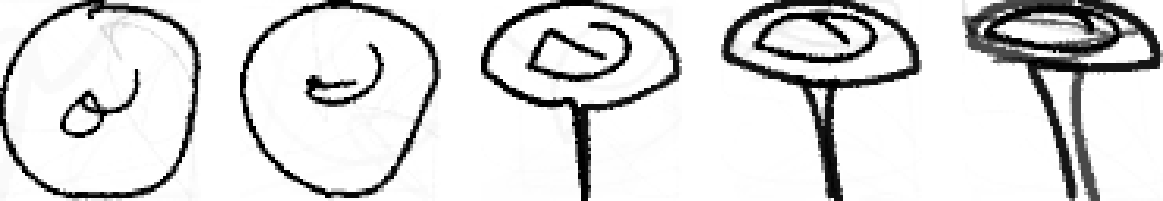
\includegraphics[width=0.45\linewidth]{images/my_plot_raster.png}
\end{center}
\end{block}
	

\begin{columns}[T]

%%%% First Column
\begin{column}{.33\textwidth}

\begin{block}{Abstract}
\textbf{Vector graphics} allows for editing without loss of quality. It stores images as a collection of primitives (lines, bezier curves, circles, etc.) with corresponding properties (size, width, control points).

\textbf{Typical generative models} are trained on raster images, while vector graphics space is non-euclidean. Several approaches were tried, until finally a differentiable rasterizer proposed in \cite{diffsvg} made it possible to do a direct backpropagation to svg parameters. 
\linebreak
\linebreak
\textbf{In this project} we apply differentiable rasterizer from \cite{diffsvg} to experiment with generative art on different datasets, GAN architectures, and create adversarial examples using painting.

\end{block}

\begin{block}{Related work}
	Most generative adversarial networks are generating raster images. DoodlerGAN \cite{doodlergan} aimed to replicate human drawings by generating raster body parts.
	
	\paragraph{SketchRNN} \cite{sketchrnn} modeled drawing as a decision making sequential process and trained seq2seq RNN VAE to generate quick sketches. SVG VAE \cite{svgvae} applies the same approach to model fonts as a sequence of 4 commands, SketchBERT \cite{sketchbert} moved to a next level by training a giant BERT model on the same data. DeepSVG \cite{carlier2020deepsvg} uses transformers to generate SVG control commands for a vider family of svg primitives.

	
	\paragraph{Differentiable rasterizer} proposed in \cite{diffsvg} allows gradient flow from rendered image to svg parameteres, thus we can optimize svg primitives directly from raster signal. They also showed several application of generative models. Im2Vec \cite{reddy2021im2vec} uses this rasterizer to generate vector graphics from raster examples.
	
\end{block}

\end{column}

%%%% Second Column
\begin{column}{.3\textwidth}



\begin{block}{GAN architectures}
	Apart from playing with "vanilla" GAN (with and without convolutions) we tried the following approaches:
	
\paragraph{WGAN} \cite{arjovsky2017wasserstein} makes a critic $K$-Lipschitz by clipping its gradients to stabilize training 
$$\omega \leftarrow \text{clip} (\omega, -0.01, 0.01)$$

\paragraph {WGAN-GP} \cite{gulrajani2017improved} forces $K$-Lipschitz by adding a gradient penalty to the loss
$$\hat x \leftarrow \epsilon x_{real} + (1-\epsilon) x_{fake}$$ 
$$\text{loss} \leftarrow D(x_{fake}) - D(x_{real}) + \lambda (\| \nabla_{\hat x} D(\hat x) \|_2 - 1)^2$$
 
\paragraph {SNGAN} \cite{miyato2018spectral} Force 1-Lipschitz continuity by spectral normalization of critic's layers
$$\bar W_{SN} (W) = \frac W {\sigma(W)} $$

\paragraph {LOGAN} \cite{wu2020logan} More gradient flow to generator by making a latent gradient step $z = z + \Delta z$ before passing image to discriminator
$$g = \frac{\partial D(G(z))}{\partial z}$$
$$\Delta z = \frac {\alpha} {\beta + \| g \|^2} \cdot g$$

\paragraph{Results} LOGAN suffered from mode collapse and instabilities, and we haven't managed to make it train. 

\begin{table}[]
	\begin{tabular}{lll}
		\textbf{Model} & \textbf{IS} & \textbf{FID} \\
		WGAN           & 1.935       & 94.14        \\
		WGAN-GP        & 1.856       & 101.7        \\
		SN WGAN-GP     & 1.919       & 84.54        \\
		LOGAN NGD      & 1.11        & 208         
	\end{tabular}
\end{table}

While Inception Score and Frechet Inception Distance are good for automatic evaluation of generative models for realistic images, we found them less informative for grayscale sketches.

\end{block}



\end{column}

%%%% This is the THIRD column
\begin{column}{.33\textwidth}

\begin{block}{GAN details}
	\paragraph{Training time} Rasterization is expensive, (i.e. iterative root solving for high-degree polynomials), and it affects training. 
	
	\paragraph{Two Time-Scale Update Rule} Helped stabilize training. In simple words, the idea is to put smaller learning rate for the generator.
	
	\paragraph{Inception Score} To evaluate generation results we used two metrics. Inception score takes pre-trained inception model and measures the distribution of predicted labels over generated samples.
	
	\paragraph{Frechet Inception Distance} Evaluate feature distribution of a pre-trained inception model over real data and generated samples.
	$$\| \mu_{real} - \mu_{fake} \|_2^2 + \text{Trace}(\Sigma_{real} + \Sigma_{fake} - 2 (\Sigma_1 \Sigma_2)^{0.5})$$
	
	\paragraph{Complex dataset} We tried training VectorGAN on a dataset of complex images. It takes a lot more time to converge to meaningful drawings.
	
	\paragraph{Draw with more primitives} Discrete decisions (such as number of primitives and their types) are still non-differentiable operation. Our model works with bezier curves (x16) and circles (x5), as other primitives are rare in the dataset.
	
	\paragraph{Interpolation} Having 2 latent vectors, we can interpolate between images. Note that although model was trained on 64x64 images, we can generate image of any resolution, thanks to the vector graphics.
	\begin{center}
		
\includegraphics[width=0.7\linewidth]{images/inter1.png}
	\end{center}
	
	\paragraph{Meaningful directions} This is an area for future experiments. Now, as the generator has direct access to positions and control parameters, disentangling latent space directions seems easier. Is it really?
	\begin{center}
		
\includegraphics[width=0.7\linewidth]{images/inter2.png}
	\end{center}
	
\end{block}

\end{column}

\end{columns}

\begin{block}{Generative Art}
	
	\paragraph{Painterly rendering}
	Fit svg parameters to match with raster image. Discrete decisions (number of strokes, types) is still fixed by a human.
	\begin{center}
		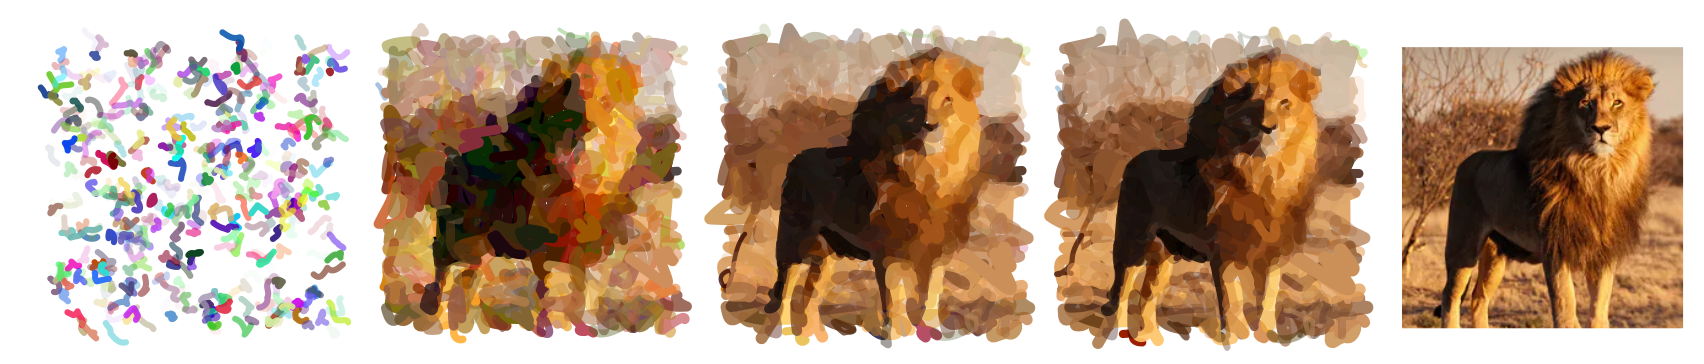
\includegraphics[width=0.6\linewidth]{images/paint_iterations.png}
	\end{center}
	
	\paragraph{Adversarial creator}
	Update parameters of svg to fool InceptionV3 into wrong classification. For example, fast gradient sign method or just plain gradient descent. We can also fix some parameters, and update only colors, or control points, or widths.
	
	Initial idea was to have small number of strokes and, starting from random, move it towards inception models gradients. However, it produces adversarial example with little artistic meaning, consider picture on the right.
	\begin{center}
		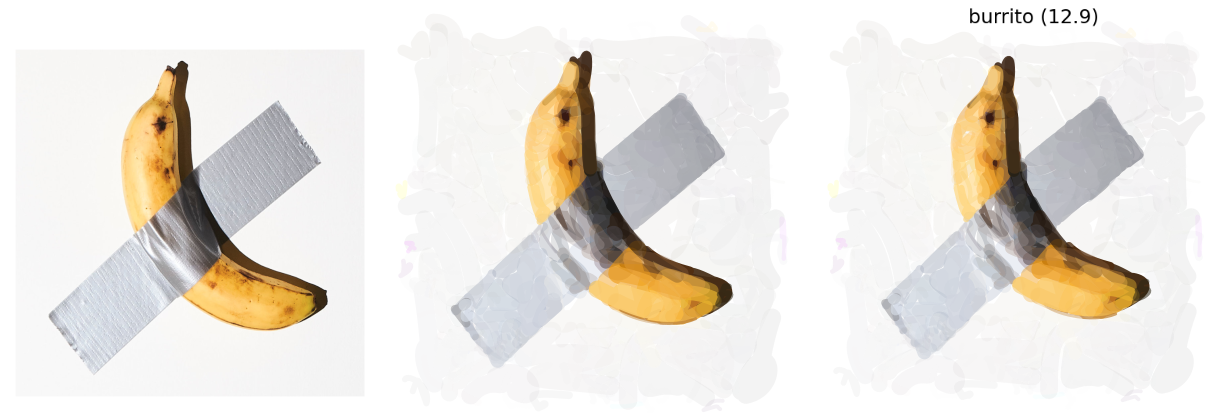
\includegraphics[width=0.45\linewidth]{images/adversarial.png}
		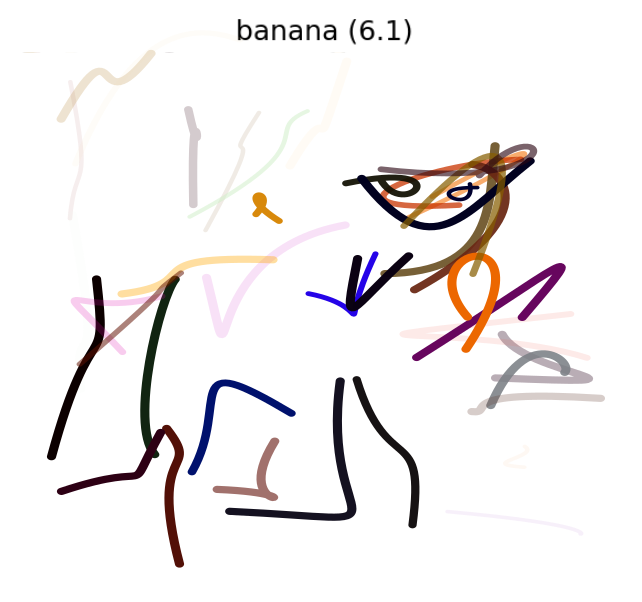
\includegraphics[width=0.16\linewidth]{images/banana.png}
	\end{center}
	
	\paragraph{Adversarial vandal}
	Draw on top of a raster picture to fool InceptionV3. Update svg parameters to maximize target class score.
	\begin{center}
		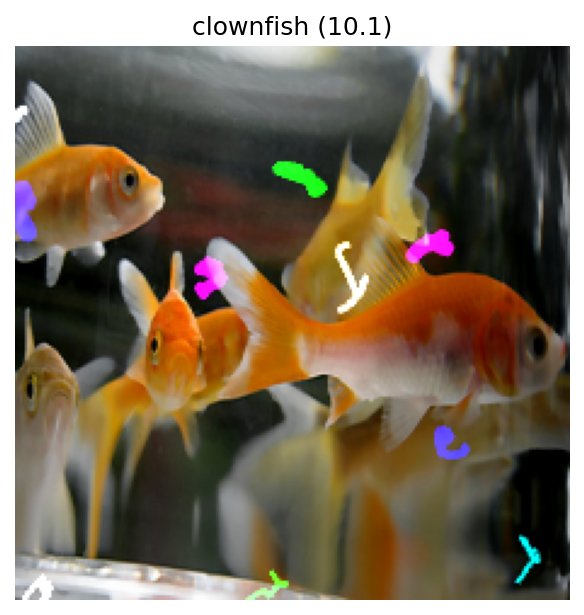
\includegraphics[width=0.15\linewidth]{images/vandal.png}
		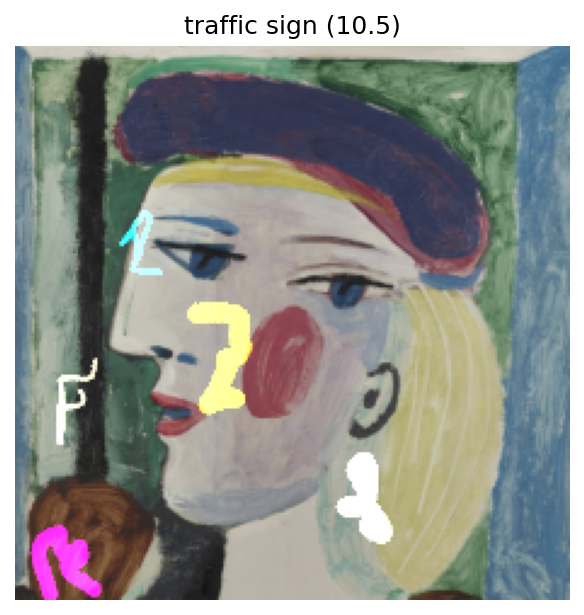
\includegraphics[width=0.15\linewidth]{images/vandal1.png}
		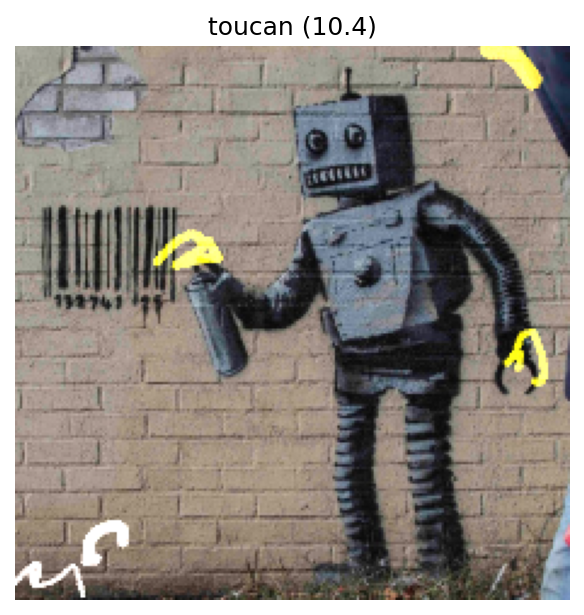
\includegraphics[width=0.15\linewidth]{images/vandal2.png}
	\end{center}
	
	
\end{block}

\begin{block}{}


\bibliography{my}


\end{block}


\end{frame}

\end{document}